\documentclass[11pt,a4paper]{article}
\usepackage[UTF8]{ctex}
\usepackage[backend=bibtex]{biblatex}
\usepackage{amsmath,amsthm,amssymb,graphicx,multirow,float,caption}
\usepackage{geometry}
\geometry{left=2.54cm, right=2.54cm, top=3.18cm, bottom=3.18cm}
\usepackage{enumitem}
\usepackage{subcaption,booktabs,diagbox}
\setenumerate[1]{itemsep=0pt,partopsep=0pt,parsep=\parskip,topsep=5pt}
\setitemize[1]{itemsep=0pt,partopsep=0pt,parsep=\parskip,topsep=5pt}
\setdescription{itemsep=0pt,partopsep=0pt,parsep=\parskip,topsep=5pt}
\usepackage{adjustbox}
\usepackage[graphicx]{realboxes}
\usepackage{rotating}

\usepackage{titlesec}

\newcommand{\be}[1]{
    \begin{equation}
        #1
    \end{equation}
}

\newcommand{\bfig}[3]{
    \begin{figure}[H]
        \centering
        \includegraphics[width=#1\textwidth]{#2}
        \caption{#3}
    \end{figure}
}

\titleformat{\section}%设置section的样式
{\raggedright\large\bfseries}%右对齐,4号字,加粗
{\thesection .\quad}%标号后面有个点
{0pt}%sep label和title之间的水平距离
{}%标题前没有内容

\title{\vspace{-4cm}\Large X射线的产生与X射线谱}  %文章标题
\author{\kaishu 学号:202111999064 \hspace{1.5cm} 姓名:郑力恒 \hspace{1.5cm} 指导老师: 王海波}   %作者的名称
\date{}

\begin{document}
\maketitle

\begin{abstract}
    本实验简要介绍了X射线的产生原理,探讨了X射线谱的规律、X射线与物质的相互作用以及X射线光谱分析方法。研究了单晶的布拉格衍射现象,发现钼靶材料对应的X射线标识谱中有两条特征峰值波长,分别为$\lambda_1=0.0617$ nm和$\lambda_2=0.0696$ nm。还研究了X射线管的电压及其对X射线谱的影响,验证了Duane-Hunt关系,并计算出普朗克常量为$h=7.352\times10^{-34}\text{J}\cdot\text{s}$,相对误差为10\%。
	
\end{abstract}

\section{引言}
1895年,德国物理学家伦琴在研究阴极射线时发现了X射线。X射线在医疗诊断和金属探伤领域具有重要应用价值,并为多种科学研究提供了一种有效的工具。

在科学家探索X射线本质的过程中,1912年劳厄等人发现了X射线在晶体中的衍射现象,证实了X射线是波长约为0.1纳米的电磁波。在进一步研究X射线的性质时,巴克拉发现X射线具有特征谱,即不同元素发出的特征X射线包含原子内部结构的信息,这对建立原子结构理论非常重要。随后,莫塞莱在巴克拉的基础上发现了元素发出的特征X射线能量与原子序数之间的关系,即莫塞莱定律。

为了研究X射线谱的规律、X射线与物质的相互作用及X射线光谱分析方法,我们在本实验中采用能谱色散技术分析X射线特征谱,验证莫塞莱定律,并测定X射线在物质中的指数衰减规律以及吸收常数在特定能量下的突变现象。

\section{原理}
\subsection{X 射线的产生及 X 射线谱}
实验室中产生X射线最常用的方法是利用X射线管,目前常用的X射线管多为高真空热阴极类型。要使X射线管产生X射线,必须满足以下条件:首先,需要一个能够产生足够数量电子的阴极和一个能够承受高速电子撞击并产生X射线的阳极靶面;其次,需要一个高真空管,以确保电子不受阻碍地运动,避免能量损失,同时保护灯丝不被氧化而烧毁;最后,需要在管两端施加高电压,使阳极为正极,阴极为负极。当高速电子撞击阳极靶面时,仅有不到1%的能量转化为X射线,绝大部分能量转化为热能,因此X射线管在工作时,阳极靶面需要进行水冷或风冷,以避免温度急剧升高。

X射线谱是指X射线强度随波长变化的关系曲线。X射线管发出的典型X射线谱可以分为两个部分:一部分是连续谱,谱线连续平滑分布,当不同动能的电子轰击靶材时,产生的连续谱形状相似,并且都有一个最短波长$\lambda_{\min}$,该波长与管电压V有关;另一部分是线状谱,谱线表现为几个尖锐的、分立的峰,这些峰值波长与X射线管的工作条件无关,只取决于靶材的化学元素,也称为特征谱。

连续谱是由轫致辐射产生的。当高速电子撞击阳极靶时,电子在与靶原子碰撞过程中损失的能量部分或全部转化为辐射能,产生的辐射称为轫致辐射。绝大多数电子会与靶物质进行多次碰撞,逐步丧失能量,直到完全耗尽。因此,轫致辐射产生的X射线谱是连续谱。此连续谱的短波极限$\lambda_{\min}$对应于入射电子在一次碰撞中失去全部动能的情况,而X射线管中的电子动能是通过X射线管电压V加速获得的,因此有
\begin{equation}
    \lambda_{\min}=\frac{hc}{eV}=\frac{1.24\times10^3}{V} nm
\end{equation}
    其中$U$的单位为伏特(V)。该方程被称为Duane-Hunt关系式,如果在实验中测量出$U$和$\lambda_{\min}$,也可以通过此公式计算普朗克常量$h$。
    
    轫致辐射的强度与阳极靶的原子序数Z有关,频率分布由入射高速电子的能量决定。实验发现,轫致辐射产生的连续谱性质与X射线管的管电压$U$、管电流$I$和靶材料这三个因素有关:
    \begin{itemize}
    \item 当管电压$U$升高时,所有波长的X射线强度都会增加,同时短波限$\lambda_{\min}$向短波方向移动,强度最高的X射线波长$\lambda_{\max}$也会向短波方向移动;
    \item 当管电压$U$不变而管电流$I$增大时,各种波长的X射线相对强度增加,但$\lambda_{\min}$和$\lambda_{\max}$不变;
    \item 如果保持管电压和电流不变,改变阳极靶材,当阳极材料的原子序数Z增加时,各种波长的X射线相对强度增加,整个曲线向上移动,但$\lambda_{\min}$和$\lambda_{\max}$均不变;
    对连续谱进行积分可以得到连续谱的强度$I_{\text{连}}$,其满足$I_{\text{连}} = k_{\text{连}} IZV^2$。
    \end{itemize}

    特征X射线是在连续X射线的基础上产生的。当管电压V提高到某一临界值后,在连续谱上会出现离散的、强度很高的线状谱。线状谱的强度受管电压影响,而峰位与管电压无关,只由阳极靶的材料决定。

特征谱的产生机制与阳极材料的原子结构有关。当靶面被高速粒子轰击时,原子可能被激发到高能级状态,这种激发态是不稳定的,会以光量子的形式释放能量,其频率满足$h\nu=E_{n_2}-E_{n_1}$。当激发态原子的不同外层电子向K层跃迁时,会产生K系辐射。其中,电子从L层跃迁到K层产生的X射线称为$\mathbb{K}_\alpha$射线,考虑到同一能级层的精细结构,跃迁产生的谱线也有相应的精细结构,按波长减小依次用数字1、2等标记。

系列实验证明,X射线特征谱的分布有以下实验规律:
\begin{itemize}
\item X射线特征谱的峰位由原子的能级结构决定,对于特定的阳极靶材料,其特征波长是确定的,与管电压和管电流等实验条件无关,也与元素的化学状态无关;
\item 只有当管电压高于临界值$V_{\text{th}}$时,连续谱才会伴有特征谱,$V_{\text{th}}$称为X射线特征谱的激发电压。不同阳极靶材料的激发电压不同,其大小由阳极靶的原子序数Z决定。例如,对于钼靶X光管,只有当电压高于20 kV时才会产生特征谱;
\item 当管电压$U$超过激发电压$V_{\text{th}}$并继续升高时,X射线特征谱的强度随管电压$U$、管电流$I$和激发电压$V_{\text{th}}$的变化规律满足以下关系:
\begin{equation}
I_{\text{特征}}=k_{\text{特征}}I(V-V_{\text{th}})^m
\end{equation}
对于K线系,$m=1.5$;对于L线系,$m=2$。
\end{itemize}

\subsection{X 射线与物质的相互作用}
X射线与物质的相互作用主要包括以下几种:
\begin{itemize}
\item 光电效应

在光子和电子的相互作用中,如果光子的能量大于或等于原子核对电子的束缚能,电子就可能吸收光子的全部能量并被电离,成为自由电子。

\item 康普顿散射

当X射线与原子中的价电子或自由电子相互作用时,由于能量和动量守恒,散射后的出射光子的波长变化满足以下公式:
\begin{equation}
\Delta\lambda=\dfrac{h}{m_ec}(1-\cos\theta)
\end{equation}


\item 相干散射
\item 
当入射X射线与原子中束缚较强的电子相互作用时,电子在入射X射线的交变电场作用下将围绕其平衡位置振动,振动频率与入射X射线的频率相同,并向四周发射与其振动频率相同的电磁波。这种散射X射线的波长和频率均与入射X射线相同,在相同的传播方向上可以发生干涉现象,因此称为相干散射。

当X射线在晶体中与各原子的电子发生相干散射时,由于晶体中原子的排列是有规律、周期性的,且原子间距与X射线波长相近,相干散射波在特定方向上会发生干涉,从而产生衍射线。晶体的衍射方向取决于晶体微观结构的类型及其基本尺寸(如晶面间距、晶胞参数等);衍射线的强度取决于晶胞中各组成原子的元素种类及其排列的坐标。

如图1所示,晶体相邻晶面上反射的X射线光程差为$\delta=2d\sin\theta$,当$\delta$为入射X射线波长$\lambda$的整数$n$倍时
\begin{equation}\label{eq
}
2d\sin\theta=n\lambda,\quad n\in\mathbb{Z}
\end{equation}
将产生第$n$级干涉极大,该方程称为布拉格方程。
\end{itemize}
\begin{figure}[H]
\centering
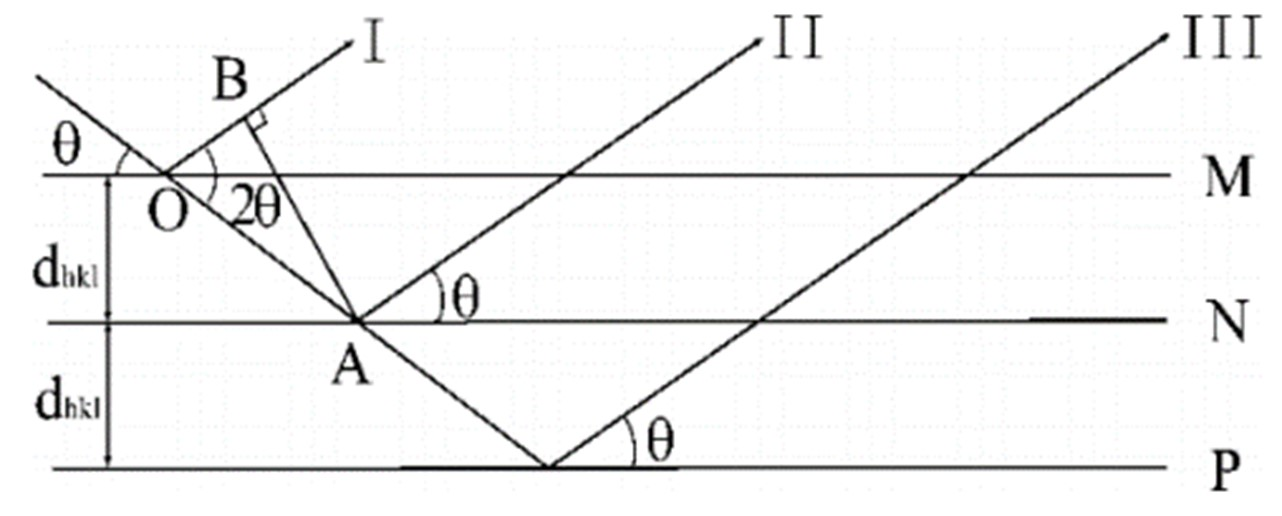
\includegraphics[scale=0.4]{1.jpg}
\captionsetup{font=footnotesize}
\caption{X射线在晶面族上的衍射}
\end{figure}

\subsection{X射线衍射仪}
X射线衍射仪通常由X射线发生器、测角仪及控制系统、X射线探测器以及相应的数据采集和处理分析软件组成。其结构示意图如图2所示。X射线管发出的X射线经过光阑准直后照射到待测样品上,衍射线通过探测器采集。样品台和探测器支架分别装在测角仪的两个同轴转盘上,以$\theta:2\theta$的方式连动,以记录不同方向上的衍射线强度。测角仪是衍射仪中最精密的机械部分,也是衍射仪的核心。

\begin{figure}[H]
\centering
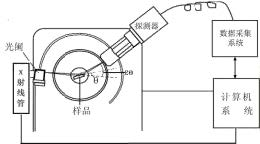
\includegraphics[scale=0.7]{2.jpg}
\captionsetup{font=footnotesize}
\caption{X射线衍射仪结构示意图}
\end{figure}

\section{实验步骤}

\begin{itemize}
    \item 单晶的布拉格衍射研究
    
    检查仪器无误后,安装氯化钠单晶样品:带手套操作,仅接触样品短边;固定时轻轻卡住。
    
    设置X射线管工作条件:高压$U=35$ kV,电流$I=1.00$ mA,按(COUPLED)按钮,选择样品臂与探测臂耦合扫描方式,设置$\beta_{\min}=2^\circ,\beta_{\max}=25^\circ$, 步幅$\Delta\beta=0.1^\circ$,各角度测量时长$\Delta t=10$秒,然后按仪器控制区下方的“SCAN”按钮等待扫描。
    
    \item 研究X射线管的电压对于X射线谱的影响
    
    设置$U=15$ kV,$I=1$ mA,$\beta_{\min}=2^\circ,\beta_{\max}=10^\circ$,其余设置不变然后扫描。
    
    隔5 kV改变一次电压,直至35 kV,其余设置不变并扫描,保存数据和曲线并分析。
    

    \item 研究X射线管的电流对于X射线谱的影响
    
    设置$U=35$ kV, $I=0.4$ mA,$\beta_{\min}=6^\circ,\beta_{\max}=7.5^\circ$。隔$0.1$ mA改变一次电流,直至$1$ mA,其余设置不变并扫描,保存数据和曲线并分析。
    \end{itemize}

\section{结果分析与讨论}
\subsection{单晶布拉格衍射}
根据图3,在$\beta:2^\circ \sim 25^\circ$范围内可以看到六个衍射峰,对应三个衍射级次。选取$U=35 $kV的谱线并结合式(\ref{eq
})计算得衍射波长如下表所示($d=0.282 $nm)。

\begin{table}[H]
    \centering
	\caption{X射线谱特征波长计算}
        \begin{tabular}{|c|cccccc|}
        \hline
        n       & \multicolumn{2}{c|}{1}                                    & \multicolumn{2}{c|}{2}                                    & \multicolumn{2}{c|}{3}               \\ \hline
        $\beta$   & \multicolumn{1}{c|}{6.3°}   & \multicolumn{1}{c|}{7.1°}   & \multicolumn{1}{c|}{12.6°}  & \multicolumn{1}{c|}{14.2°}  & \multicolumn{1}{c|}{19.2°}  & 21.8°  \\ \hline
        $\lambda_1$/nm & \multicolumn{1}{c|}{0.0619} & \multicolumn{1}{c|}{}       & \multicolumn{1}{c|}{0.0615} & \multicolumn{1}{c|}{}       & \multicolumn{1}{c|}{0.0618} &        \\ \hline
        $\lambda_2$/nm & \multicolumn{1}{c|}{}       & \multicolumn{1}{c|}{0.0697} & \multicolumn{1}{c|}{}       & \multicolumn{1}{c|}{0.0692} & \multicolumn{1}{c|}{}       & 0.0698 \\ \hline
        $\overline{\lambda_1}$/nm & \multicolumn{6}{c|}{0.0617}                                                                                                                                  \\ \hline
        $\overline{\lambda_2}$/nm & \multicolumn{6}{c|}{0.0696}                                                                                                                                  \\ \hline
        \end{tabular}
        \end{table}

该阳极材料对应的X射线特征谱只有两条峰值波长,分别为:
\begin{equation}
\begin{aligned}
\lambda_1 &= 0.0617\text{nm} \\
\lambda_2 &= 0.0696\text{nm}
\end{aligned}
\end{equation}
\begin{figure}[H]
    \centering
    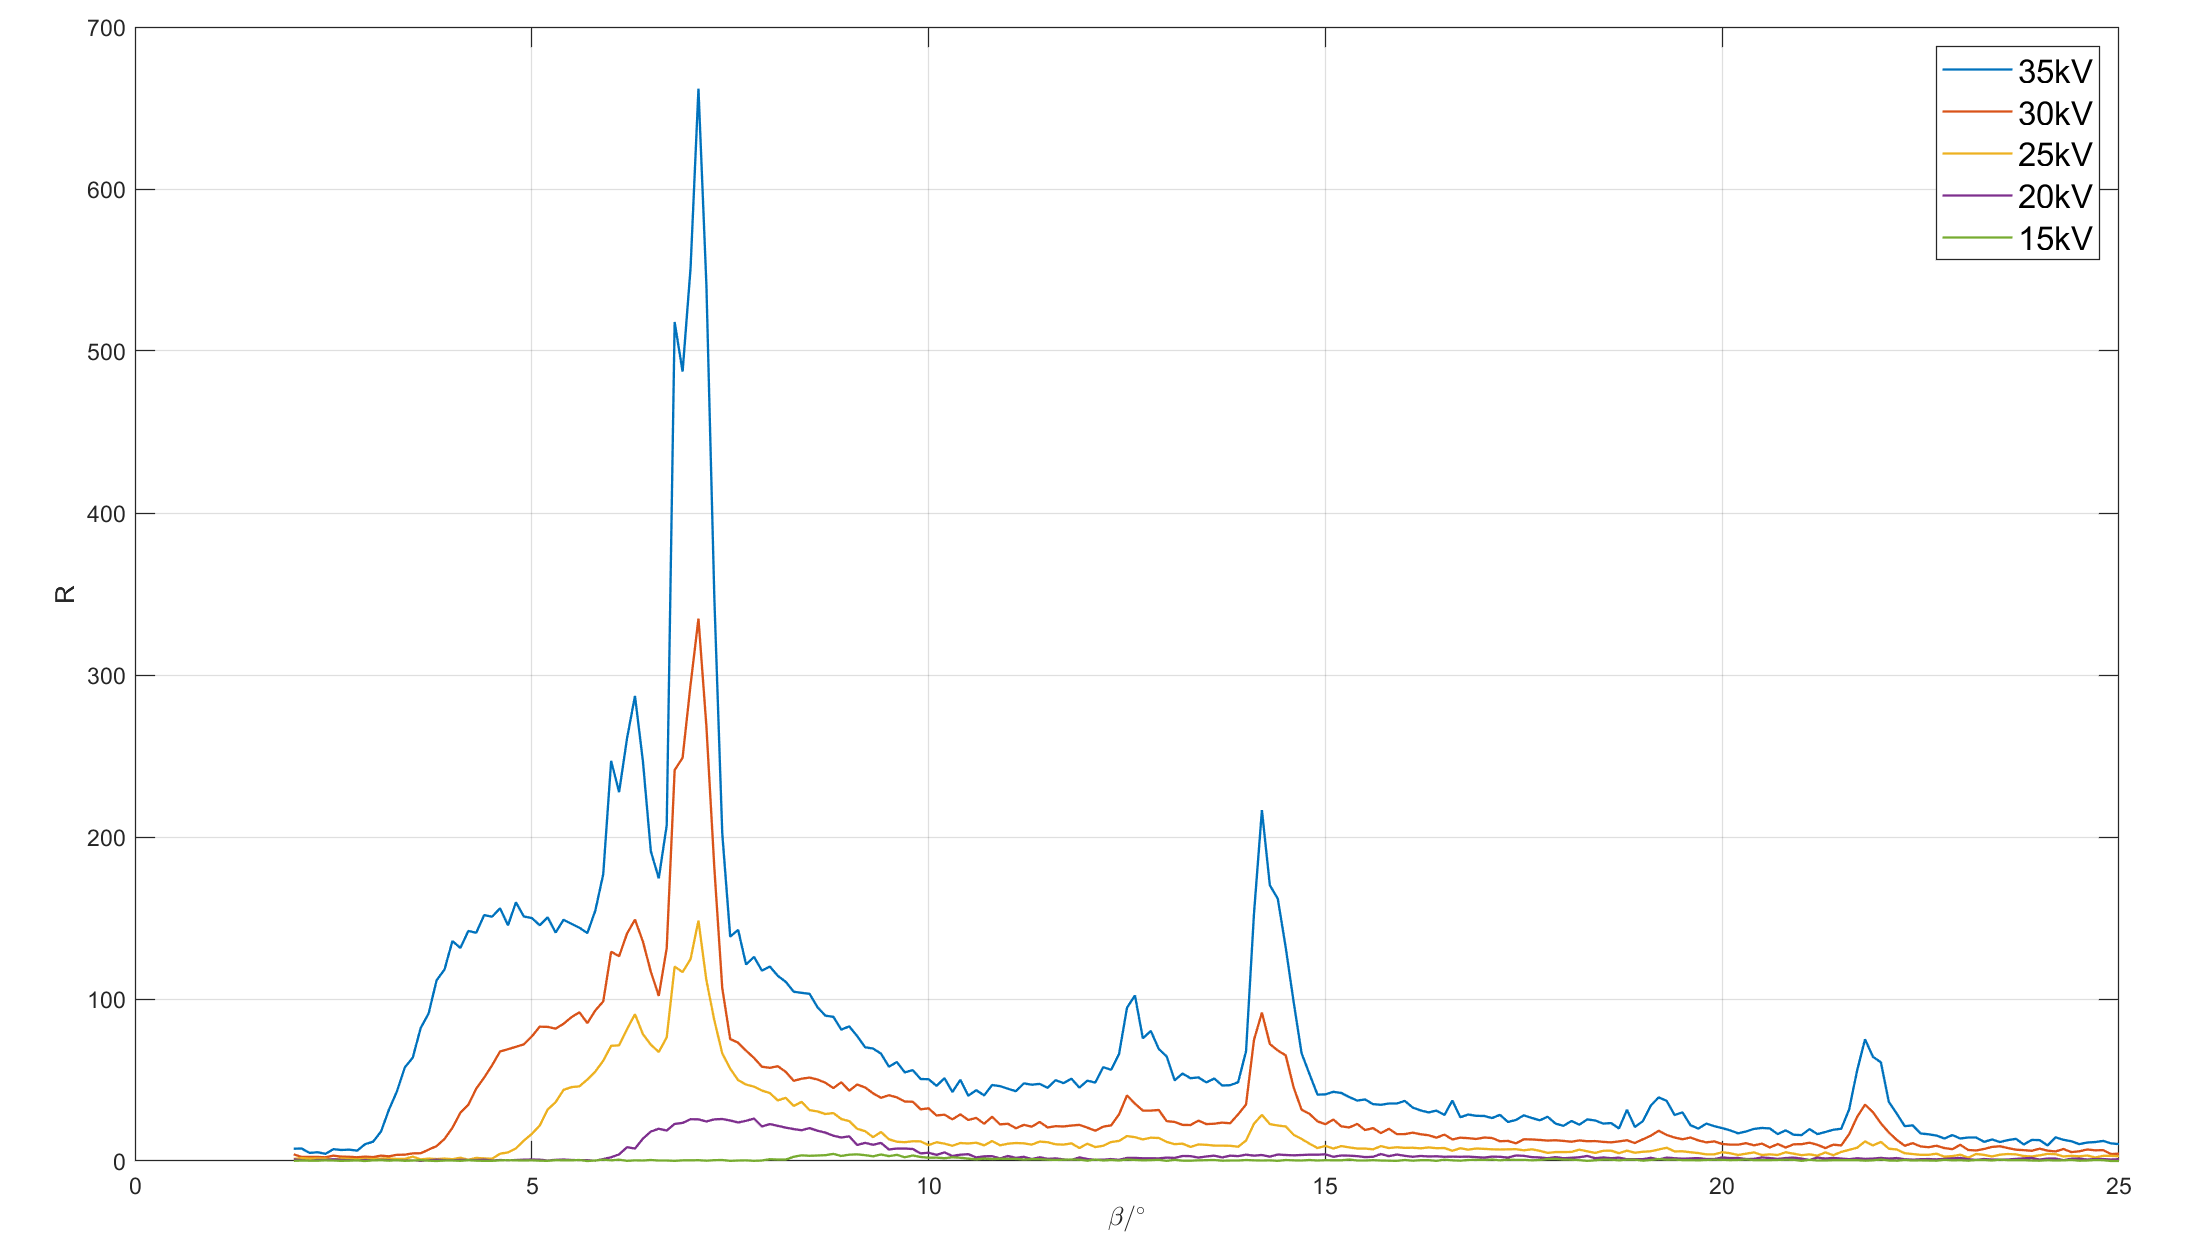
\includegraphics[width=1\textwidth]{voltage.png}
    \captionsetup{font=footnotesize}
    \caption{从上到下电压为$35, 30, 25, 20, 15$ kV对应相对强度随样平台相对初始平行线转过角度$\beta$的变化情况}
    \end{figure}
    
    接着改变电压大小,并保持电流$I=1$ mA不变,本次实验测量了在电压$15\sim35$ kV范围内的五条衍射谱线。通过分析,我们得出以下结论:
    
    \begin{itemize}
    \item 针对连续谱,从图3可以看到,随着管电压$U$的升高,所有波长的X射线强度均增加,同时短波限$\lambda_{\min}$向短波方向移动。
    \item 针对特征谱,我们可以看到,改变电压后峰值波长对应的样平台转过角度不变,即峰值波长不变,说明X射线特征谱的峰位与管电压无关。
    \item 图3中只有最上面的三条谱线同时具有连续谱和特征谱,而在$U=15$ kV和$20$ kV时,X射线只有连续谱。这表明,只有当管电压高于临界值$V_{\text{th}}$时,连续谱才会伴有特征谱。
    \end{itemize}
    
    在实验的初次测量时,峰值波长的强度非常小。调整了样平台与探测器之间的距离,并重新放置样品后,峰值波长的强度增加了10倍,但与图3的最大值仍有10倍的差距。这主要是由于测试角度的问题,探测器与样平台相对初始平行线之间的角度不严格呈$2:1$的关系,大部分对应角度的X射线并未被探测器检测到。在软件校准之后,角度得到校准,相应角度的X射线基本被检测到,所测强度也接近真实该角度的X射线强度。
    
    总结误差分析如下:
    
    角度测量精度不足,步幅$\Delta\beta=0.1^\circ$,测量出的角度并非严格的峰值,这是主要的误差来源。
    出射光为非平行光,出射口和探测口存在一定的宽度,带来测量上的一些误差,但这不是主要因素。

    \subsection{Duane-Hunt关系验证与普朗克常量计算}
本节通过比较Duane-Hunt关系和布拉格衍射方程计算的短波限$\lambda_{\min}$,验证了Duane-Hunt关系的正确性,并利用实验数据计算了普朗克常量。
实验中,我们在15 kV到35 kV的电压范围内,使用两种方法计算了短波限$\lambda_{\min}$。结果如表1所示:
\begin{table}[H]
 \centering
    \caption{利用Duane-Hunt关系和布拉格方程计算短波极限$\lambda_{\min}$}
    \begin{tabular}{|c|c|c|c|c|c|}
    \hline
    U         & 35     & 30     & 25     & 20     & 15     \\ \hline
    $\theta$     & 2.9°   & 3.7°   & 4.8°   & 6.1°   & 8.3°   \\ \hline
    $\lambda_{brg}$ & 0.0354 & 0.0413 & 0.0496 & 0.0620 & 0.0827 \\ \hline
    $\lambda_{dh}$  & 0.0285 & 0.0364 & 0.0472 & 0.0599 & 0.0814 \\ \hline
    \end{tabular}
    \end{table}
    需要注意的是,在15 kV电压下,峰值相对强度较低,可能导致较大误差。
    \begin{figure}[H]
    \centering
    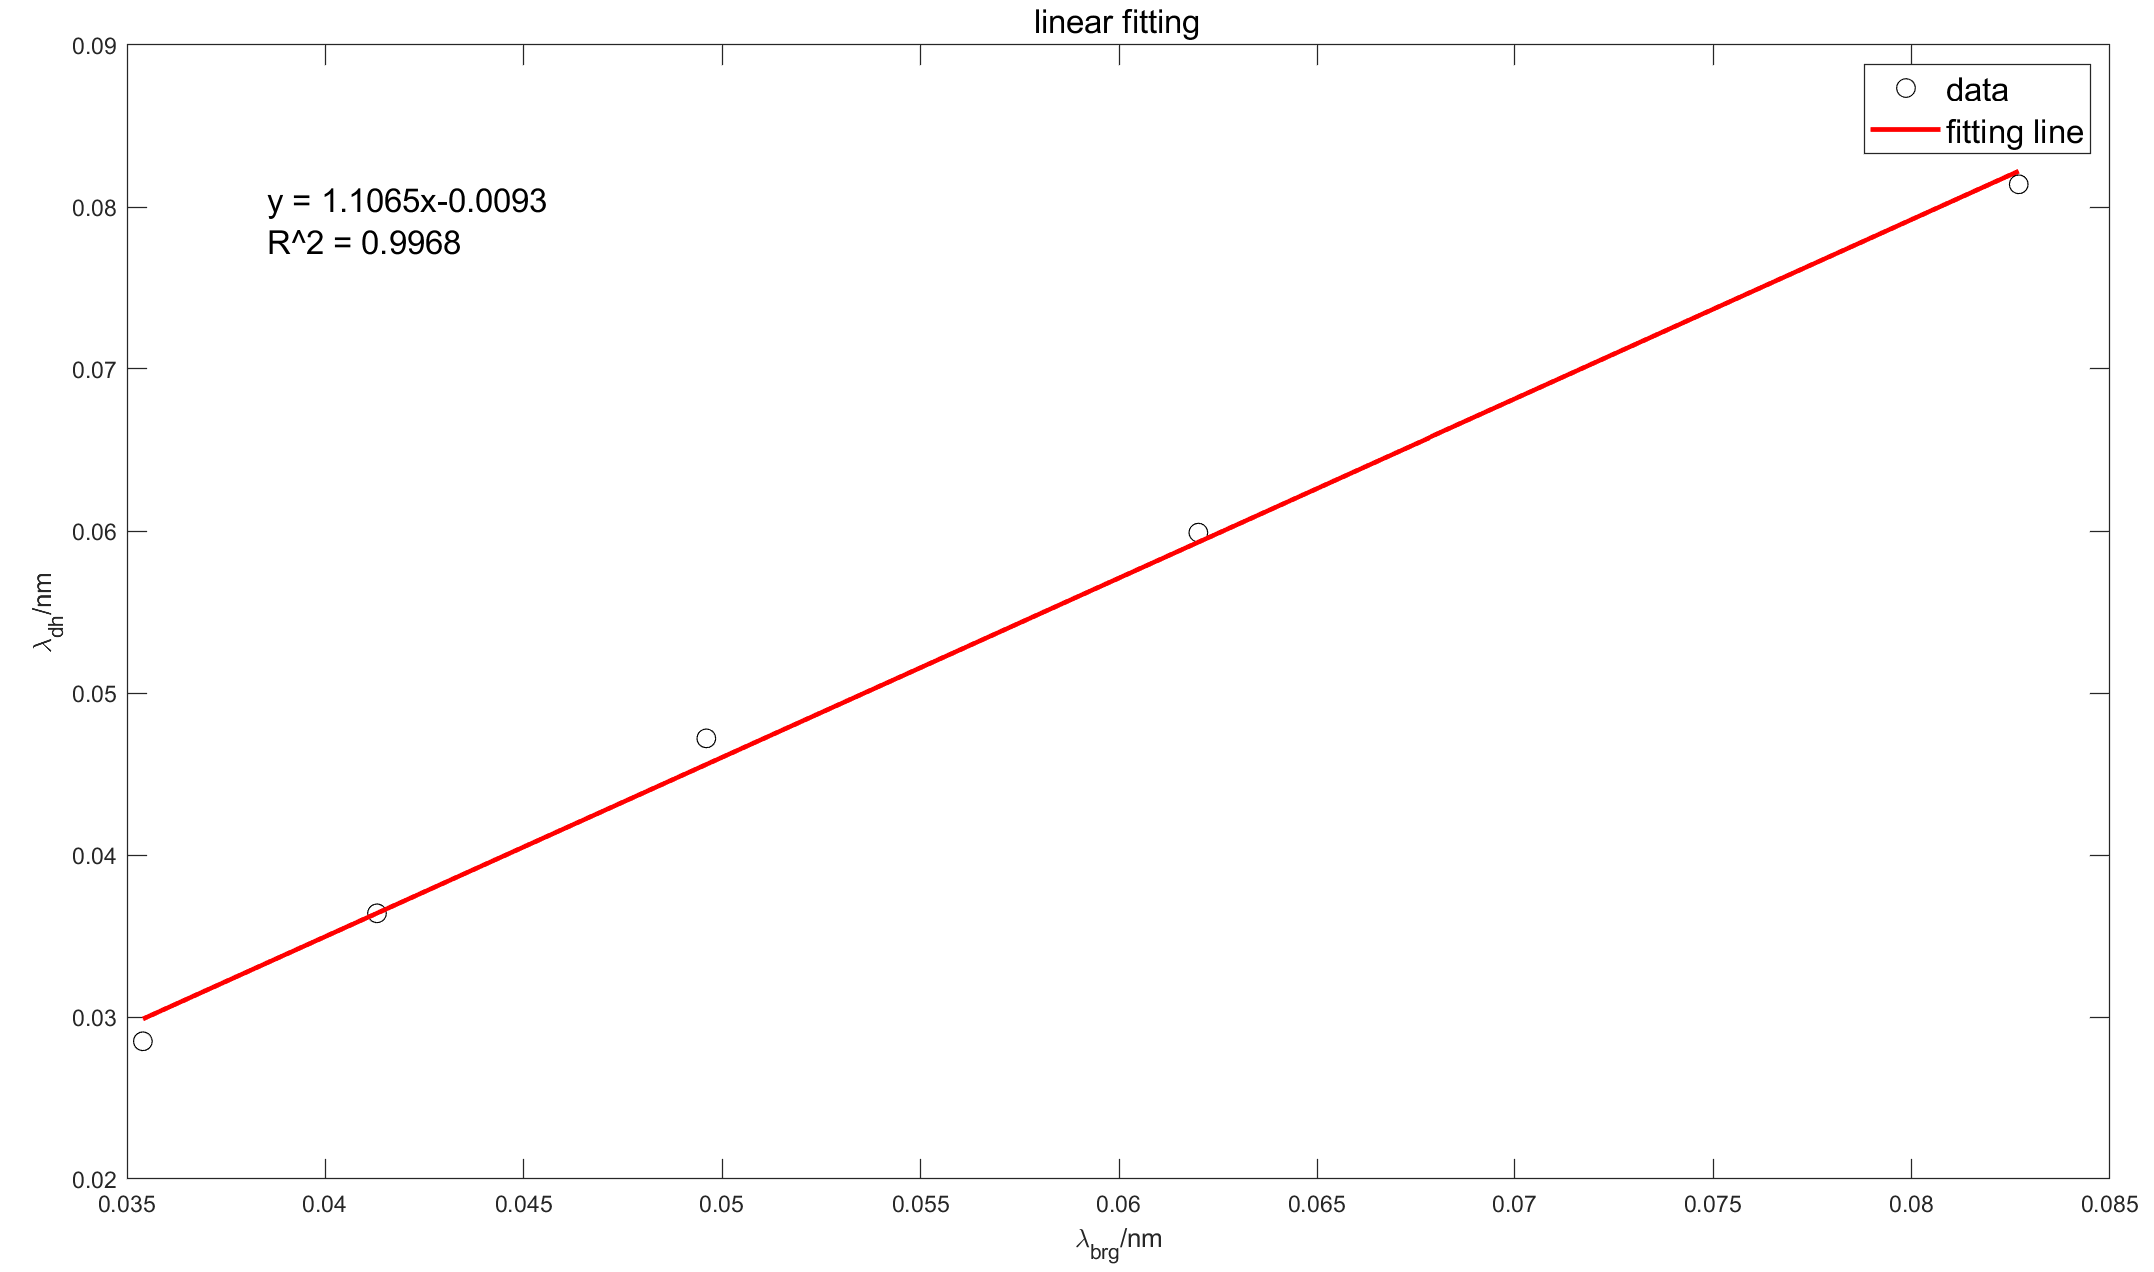
\includegraphics[scale=0.5]{dh_brg.png}
    \captionsetup{font=footnotesize}
    \caption{Duane-Hunt关系与布拉格方程计算的$\lambda_{\min}$对比}
    \end{figure}
    如图1所示,我们使用Matlab进行线性拟合,得到:
    \begin{equation}\label{eq:fitting_dh}
    \lambda_{\text{dh}}=1.1065\lambda_{\text{brg}}-0.0093(nm),\qquad R^2=0.9968
    \end{equation}
    拟合结果表明,在实验误差范围内,$\lambda_{\text{brg}}\approx\lambda_{\text{dh}}$,验证了Duane-Hunt关系的正确性。
    接下来,我们研究了短波极限$\lambda_{\min}$与X射线管电压$U$倒数的关系:
    \begin{figure}[H]
    \centering
    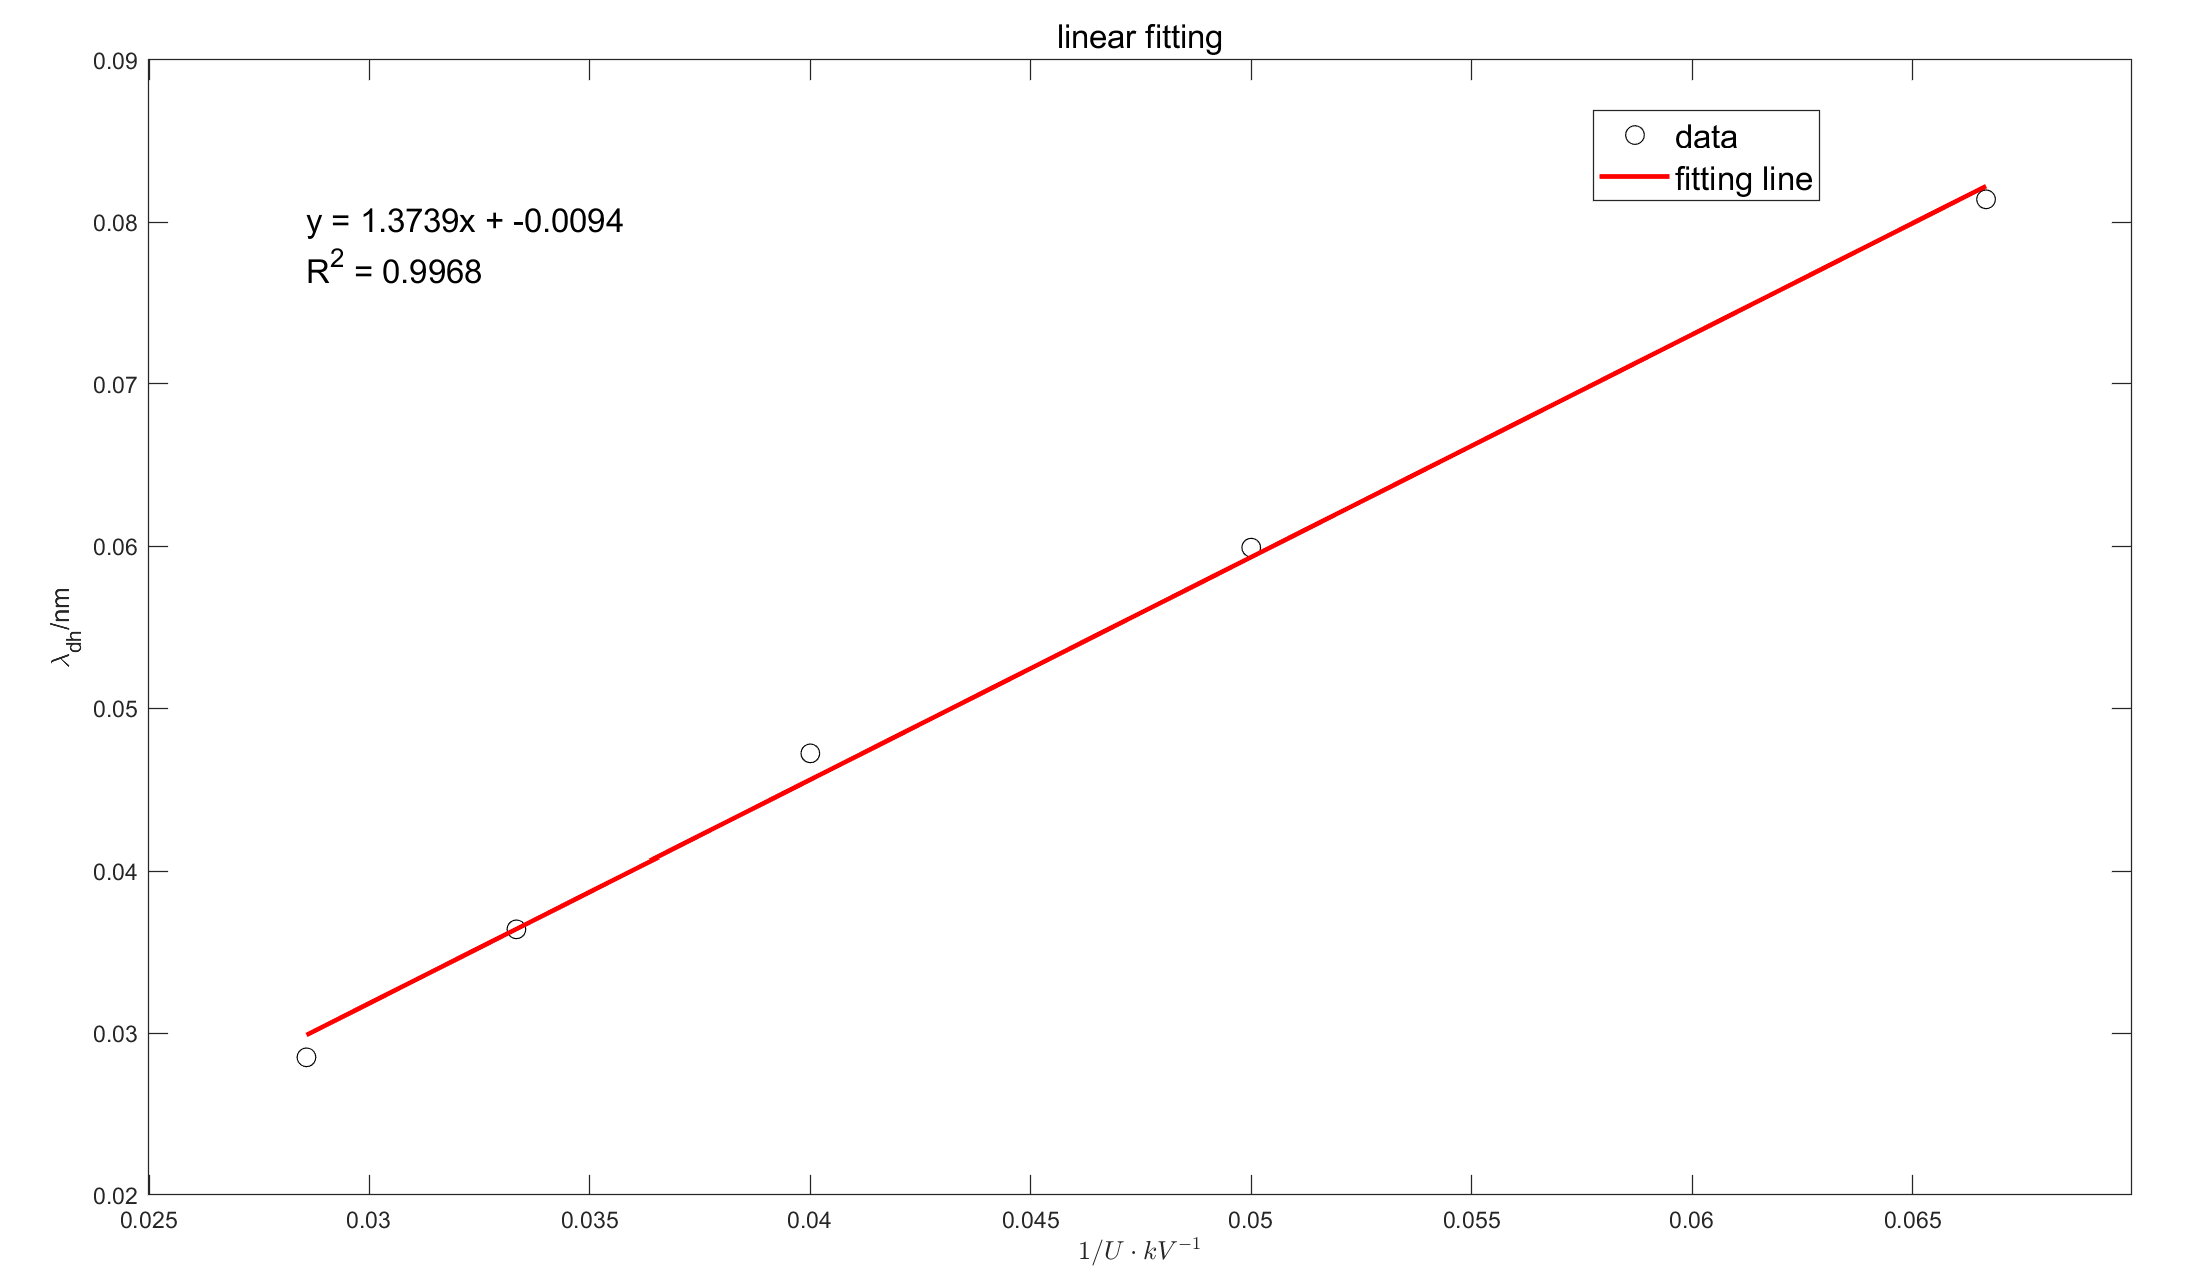
\includegraphics[scale=0.45]{lu.png}
    \captionsetup{font=footnotesize}
    \caption{短波极限$\lambda_{\min}$与X射线管电压$U$倒数的关系}
    \end{figure}
    通过线性拟合,我们得到:
    \begin{equation}
    \lambda_{\min}=\dfrac{1.3739\text{kV}}{U}-0.0094 (nm),\qquad R^2=0.9963
    \end{equation}
    拟合结果显示$\lambda_{\min}$与$1/U$近似成正比,比例系数$k=1.3739\text{kV}\cdot nm$。利用此结果,结合光速$c$和电子电荷量$e$,我们计算得到普朗克常量:
    \begin{equation}
    h=\dfrac{ek}{c}=7.352\times10^{-34}\text{J}\cdot\text{s}
    \end{equation}
    与实际值$h_{\text{re}}=6.62607015\times10^{-34}\text{J}\cdot\text{s}$相比,相对误差为$\delta=10\%$。
    实验中的主要误差来源包括:
    \begin{itemize}
    \item 角度测量精度有限(步幅$\Delta\beta=0.1^\circ$),测得的角度可能不是严格的峰值。
    \item 短波极限附近的相对强度极小,噪声影响显著,导致人工选择短波极限对应角度时存在极大误差。
    \end{itemize}
    这些因素是造成最终结果误差的主要原因。
    
    \subsection{X射线管电流对X射线谱的影响研究}
    为了研究X射线管电流对X射线谱的影响,我们在保持管电压恒定的情况下,改变电流值并观察X射线谱的变化。实验结果如图7所示。
    \begin{figure}[H]
    \centering
    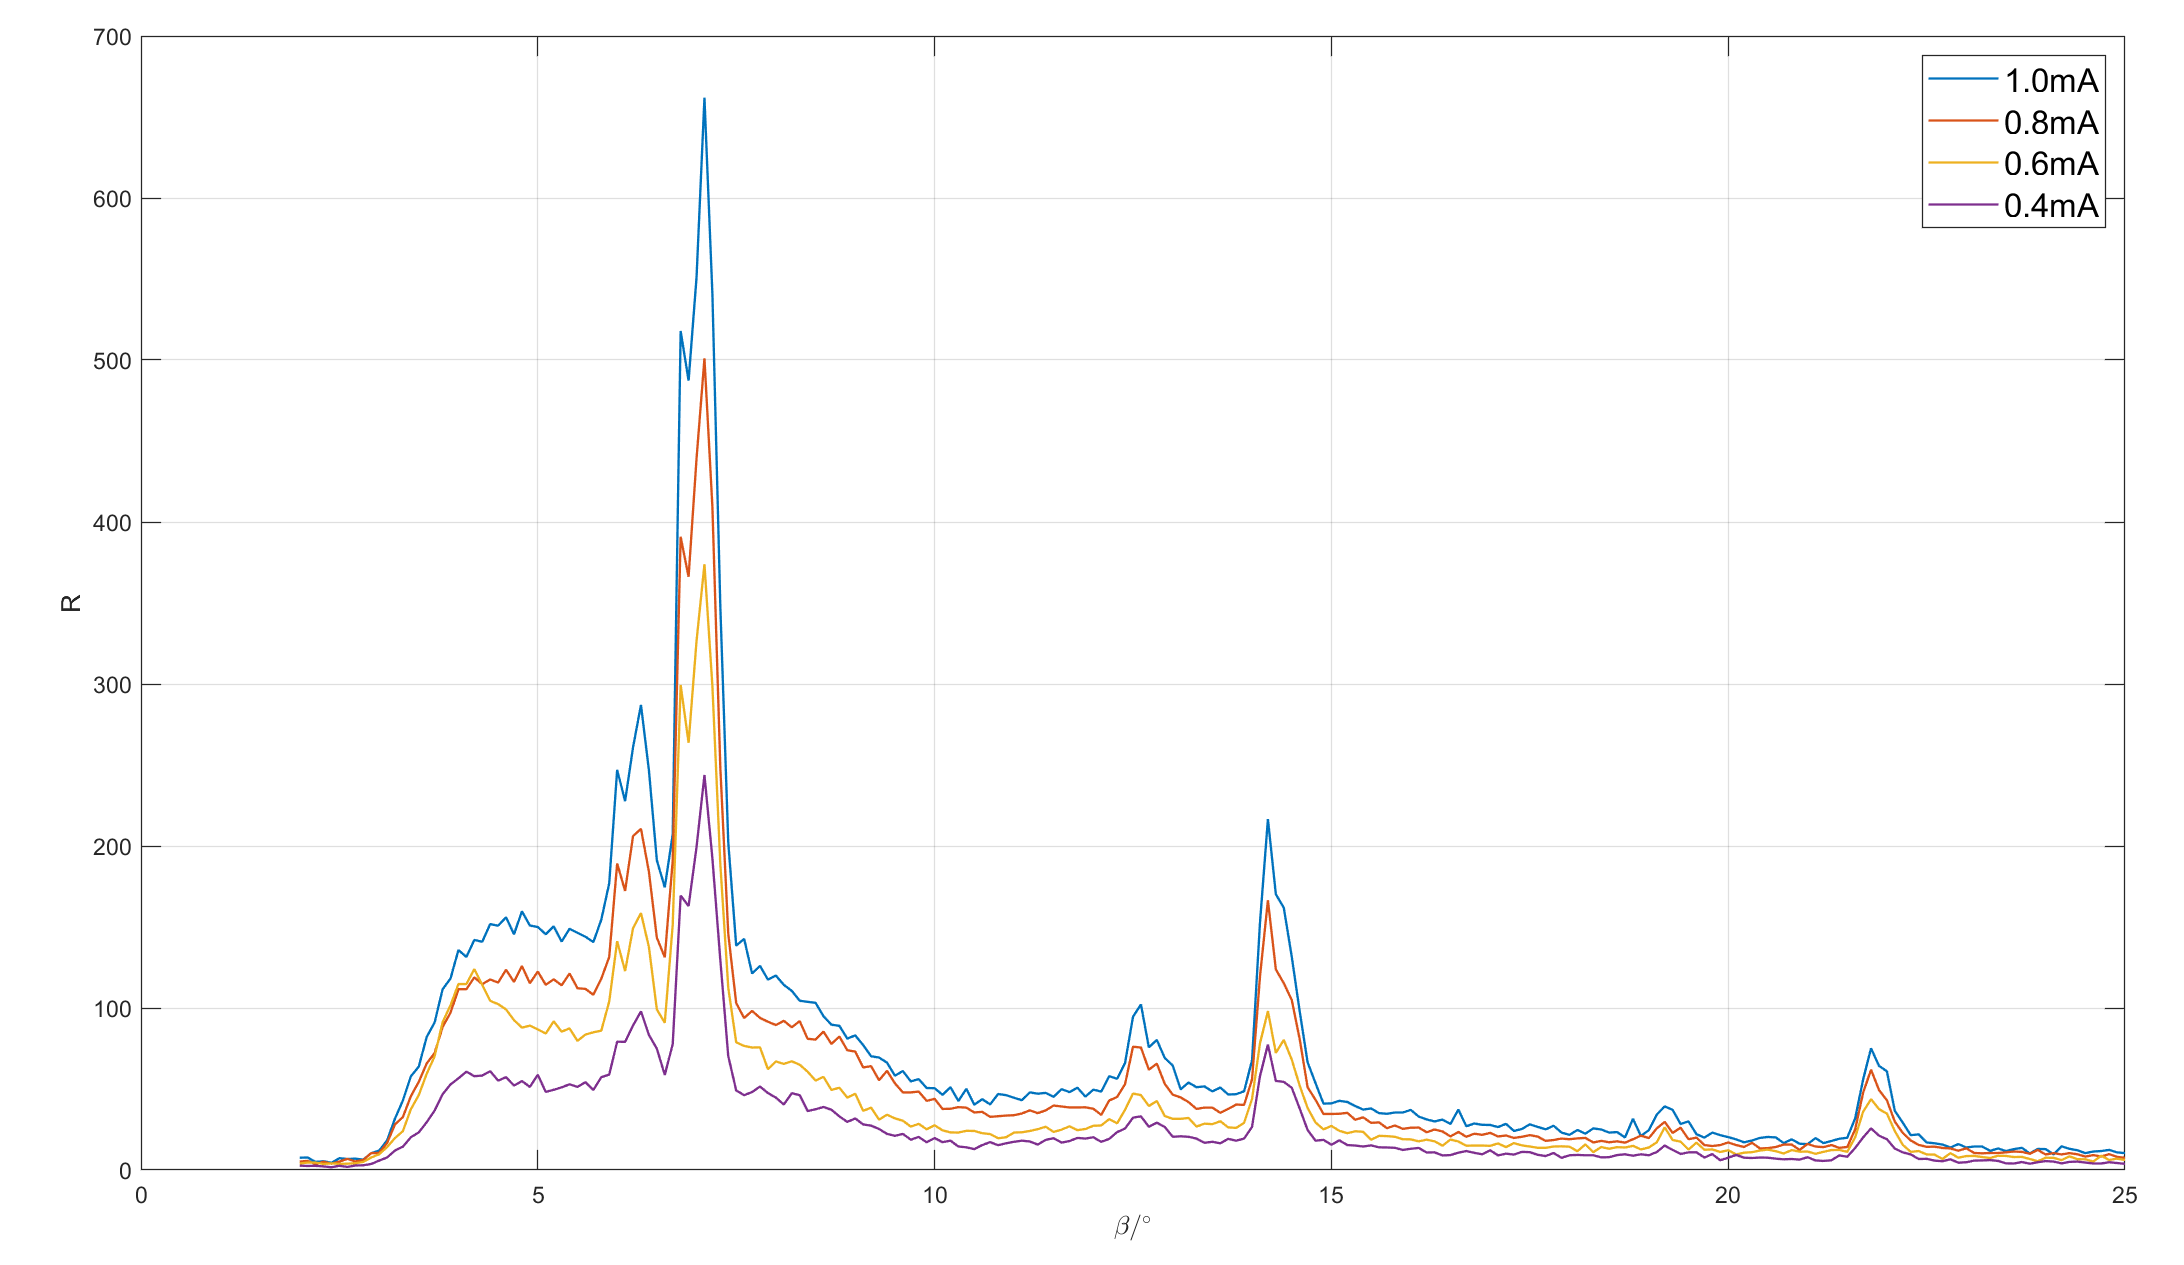
\includegraphics[width=\textwidth]{current.png}
    \captionsetup{font=footnotesize}
    \caption{不同电流下X射线相对强度随样品平台旋转角度$\beta$的变化(从上到下电流依次为1, 0.8, 0.6, 0.4 mA)}
    \end{figure}
    根据图7的实验结果,我们得出以下观察结论:
    \begin{itemize}
    \item 在固定管电压$U=35$ kV的条件下,随着管电流$I$的增大,各波长X射线的相对强度均有所增加。
    \item 对于特征谱线,改变电流不会影响峰值波长对应的样品平台旋转角度$\beta$。这表明峰值波长$\lambda$保持不变,即X射线特征谱的峰位与管电流无关。
    \end{itemize}
    \section{总结}
    本实验通过X射线衍射仪研究了单晶的布拉格衍射,主要结果如下:
    \begin{itemize}
    \item 钼靶材料的X射线特征谱包含两个峰值波长:$\lambda_1=0.0617$ nm和$\lambda_2=0.0696$ nm。
    \item X射线管电压对X射线谱的影响:
    
    连续谱:随管电压升高,所有波长的X射线强度增加,短波限$\lambda_{\min}$向短波方向移动。

    特征谱:X射线特征谱峰位与管电压无关。
    
    \item 根据实验数据计算得出普朗克常量$h=7.352\times10^{-34}\text{J}\cdot\text{s}$,相对误差为10\%。
    \item X射线管电流对X射线谱的影响:
    
    增大管电流$I$会导致各波长X射线的相对强度增加。

    X射线特征谱峰位与管电流无关。
    \end{itemize}
    
    
    这些发现深化了我们对X射线产生机制及其特性的理解,为进一步研究和应用X射线技术奠定了基础。
\end{document}